\section{Introduction} \label{sec:introduction}
Floating offshore wind turbines (FOWTs) have been the subject of numerous studies due to the possibility of exploiting the vast wind resources located in deep waters. As an emerging technology, the growth of the wind energy industry depends on FOWTs achieving more competitive costs, which has pushed for larger rotors and new designs for both floaters and moorings.

Since FOWTs are complex structures, their design requires the evaluation of performance and structural integrity for a myriad of environmental conditions (wind, wave, current, among others) and operating conditions (power production, normal shut down, fault conditions, etc.). Due to their intricate dynamics, this procedure requires modeling software capable of accounting for the couplings between aerodynamics, hydrodynamics, controls, moorings and structural behavior, which are commonly referred as aero-hydro-servo-elastic tools. A substantial effort has been made to validate these software, as exemplified by the OC3~\citep{jonkman2010report}, OC4~\citep{OC42014} and OC5~\citep{OC52017} projects, but this is still an ongoing development.

In fact, the experiments required to validate the numerical tools, usually performed in model scale, are far from an easy task, for it is impossible to keep all the dimensionless parameters that describe the different physical aspects of the problem. For instance, while the scaling of the waves requires that the Froude number ($\textrm{Fr} = U^{2}/(gL)$, with $U$ a characteristic speed, $L$ a characteristic length and $g$ the gravitational acceleration) be conserved, the aerodynamic loads are governed by the Reynolds number ($\textrm{Re} = UL/\nu$, with $\nu$ the kinematic viscosity). To work around this incompatibility, some alternatives have been tried to perform tests with both wind and waves, and a thorough review of experimental techniques for doing so can be found in \citet{otter2022review}. For instance, some works have used a Froude scaled rotor with  the wind generated by fans at higher speeds than the scaled ones, so that the correct rotor thrust was obtained \citep{martin2014methodology, skaare2007integrated, mortensen2018experimental}; however, this approach has the downside that either the tip speed ratio (TSR) or the excitation frequencies are not preserved. Others have employed performance scaled rotors \citep{goupee2014experimental, de2014development, bredmose2017triple}, in the sense that the rotors were redesigned with geometrically modified airfoils to compensate for the low Reynolds number obtained in a Froude scale experiment. 

A different line of thought is adopted by the so-called hybrid tests, in which either the aerodynamic or hydrodynamic forces are computed numerically and applied to the FOWT instead of being a consequence of the physical interaction of the hull/rotor with the waves/wind. The present work deals with the case in which the experiments are performed in a wave basin, so the waves are still generated physically, while the aerodynamic forces are replaced by a numerical model. This approach, called software-in-the-loop (SIL), was first employed by \citet{azcona2014aerodynamic}, who used a single ducted propeller in place of the turbine rotor to emulate the aerodynamic thrust, while the aerodynamic forces acting on the other degrees of freedom were disregarded. In a nutshell, it consists in measuring the motions of the FOWT model, which is floating in the wave basin, and feeding these motions to the software, in which the aerodynamic forces acting on a virtual rotor under the action of a virtual wind are computed numerically -- in that case and in the present work, using Blade Element Momentum Theory (BEMT). Finally, the rotational speed of the fan is controlled in order to provide the required thrust. The fact that this procedure happens in real time and taking into account the motions of the structure makes it simple to synchronize wave elevation and wind loads, besides allowing the modeling of aerodynamic damping and turbine control. In subsequent works, the SIL method has been applied with multi-propeller actuators in order to model not only the aerodynamic thrust, but also the forces and moments along the other degrees of freedom \citep{pires2020inclusion, otter2020emulating}. 

Alternatively, some works have employed cables pulled by winches instead of fans to emulate the aerodynamic loads \citep{sauder2016real, bachynski2016real, thys2018real}, while the option of performing the experiment in a wind tunnel whilst the hydrodynamics of the FOWT is computed numerically is discussed by \citet{bayati2018wind} and \citet{belloli2020hybrid}. However, the SIL method proposed by \citet{azcona2014aerodynamic} has the advantage of being the simplest option in terms of required equipment for a wave basin such as the one from the Numerical Offshore Tank of the University of São Paulo (TPN-USP). 

Besides improving the capabilities of TPN-USP to be able to perform experimental tests of FOWTs under the concomitant action of wind and waves, this work aims at validating the numerical models that were used during the design of a FOWT concept developed in the context of a joint research project with Petrobras~\citep{mas2022parametric}, which illustrated in Figure~\ref{fig:intro:fowtc} and goes by the provisional name FOWTC. Due to these two different objectives, this paper is divided into two parts:
\begin{figure}[!hbtp]
	\centering
	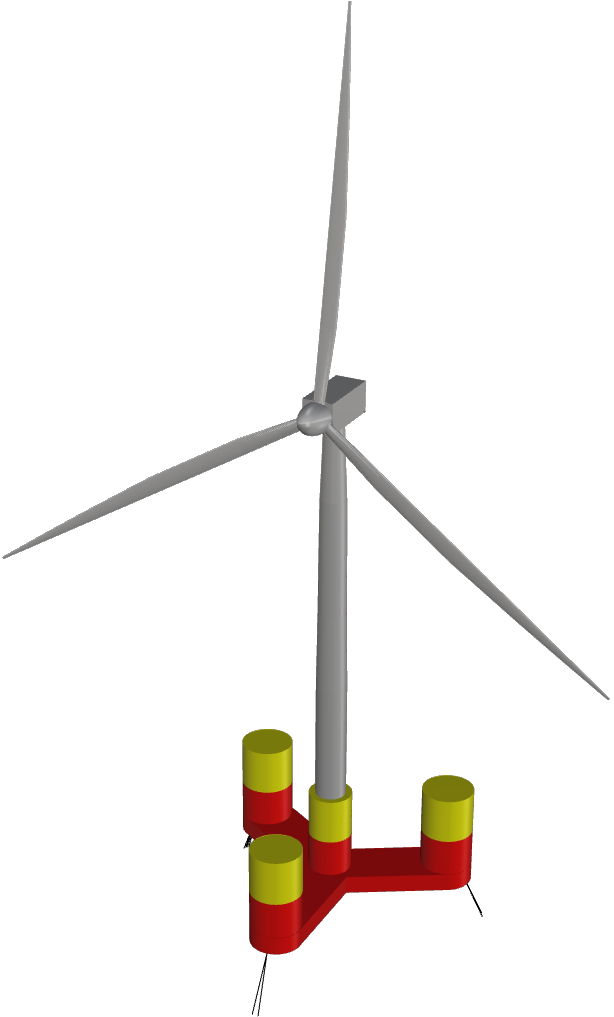
\includegraphics[scale=0.30]{./figures/Perspectiva_semfundo.png}
	\caption{Illustration of the FOWTC concept.} \label{fig:intro:fowtc}
\end{figure}

\begin{enumerate}[i.]
    \item In the first part, which is provided in Section~\ref{sec:exp_vs_num}, the experiments are used to verify aspects of the hydrodynamics of the floater (which is the part that is physically modeled in the tests) that the numerical analyses should take into account. More specifically, a numerical model as close as possible to the conditions of the experiment is built with OpenFAST~\citep{jonkman2005fast} and WAMIT~\citep{wamitManual}, and this model is used to demonstrate the importance of drag forces on the pontoons and of second-order wave forces in both the horizontal and vertical degrees of freedom (dofs). The impact of considering the mean hull inclination induced by the wind for computing the radiation/diffraction coefficients in WAMIT is also assessed, and it is shown that this effect is negligible;    
%%%%%%%%%%%%%%%%
    \item In the second part, given in Section~\ref{sec:impact_simplifications}, the objective is to investigate the relevance of two physical aspects that were not included in the aerodynamic modeling adopted in the tests. The first of them is that the SIL implementation employed a fan assembly that was only able to apply the aerodynamic thrust, thus loads in the other dofs were not present in the model; the other aspect is that blade elasticity was not considered in this first version of the software, a point that is planned to be addressed in future versions. In order to verify the impact of these simplifications, the numerical models that are validated in the first part of the paper are compared with additional OpenFAST models that consider both blade elasticity and the aerodynamic forces on the six dofs.
% (embora de forma simples com o elastodyn. Preciso estudar em que situações seria necessário usar o beamdyn).
\end{enumerate}

Before presenting the two topics above, Section~\ref{sec:description_experiment} describes the prototype and experimental setup, including the SIL method and its limitations, while Section~\ref{sec:numerical_models} describes the numerical models considered in this work. 